\section{Linear truss element theories}

\subsection{Element-Topology}

The elements used here have 2 nodes and only inherit uniaxial stress. They can thus only elongate in their axis-direction. 
\\The nodal displacements are defined as

\begin{equation}
\boldsymbol{u}^{I}=
	\begin{pmatrix}
		u_{1} \\ u_{2} \\ u_{3}
	\end{pmatrix}.
	\label{def:u}
\end{equation}

The response of the element is defined by the second order differential equation of balance of linear momentum

\begin{equation}
	\div\sigma=0\, .
\end{equation}

\subsection{Constitutive Relation}

The scalar quantity $\sigma$ denotes the uniaxial stress described by a linear elastic material, where 

\begin{equation}
	\begin{array}{ll}
		E=\text{Young's Modulus}  \\
		A=\text{Cross Section}.
	\end{array}
	\label{def:E_and_A}
\end{equation}

Furthermore, $\sigma$ is defined as

\begin{equation}
	\sigma=EA\,\varepsilon=EA\,\tilde{u}^{\prime}.
	\label{def:sigma}
\end{equation}

\subsection{Kinematics}

In the 3 methods that are used here, the nodal displacements are projected along the truss-axis with

\begin{equation}
	\tilde{u}^{I}=\,\boldsymbol{t}\cdot\boldsymbol{u}^{I}.
	\label{eq:projection}
\end{equation}

Then, the following specification for the derivative of displacements is used:

\begin{equation}
\tilde{u}^{\prime}=\dfrac{\tilde{u}^{2}-\tilde{u}^{1}}{l^{e}}.
\label{eq:u_derivative}
\end{equation}

The elemental vector of unknowns is defined as

\begin{equation}
	\boldsymbol{d}^{e}=
		\begin{pmatrix}
			u^{1}_{1} & u^{1}_{2} & u^{1}_{3} & u^{2}_{1} & u^{2}_{2} & u^{2}_{3}
		\end{pmatrix}^{T}.
\end{equation}

\subsection{Potential}
The potential of a linear truss element is given by

\begin{equation}
	\Pi = \dfrac{1}{2}\displaystyle \int_{B}EA\; \tilde{u}^{\prime \, 2}\; dx.
	\label{eq:potential_truss}
\end{equation}


In order to reach equilibrium, $\Pi$ has to become stationary, hence we state

\begin{equation}
	\dfrac{\partial\Pi}{\partial \boldsymbol{d}^{e}}=0 \, .
	\label{eq:Pi_stationary}
\end{equation}

Thus, the \textbf{R} and \textbf{K} matrices are defined as

\begin{equation}
	\textbf{R}=\dfrac{\partial\Pi}{\partial\boldsymbol{d}^{e}}  \quad \text{and} \quad \textbf{K}=\dfrac{\partial\boldsymbol{R}}{\partial \boldsymbol{d}^{e}}\, .
	\label{R_K_Potential}
\end{equation}

\subsection{Standard Galerkin Method}

Here, the second order differential equation  from (\ref{eq:potential_truss}) is transformed 
to a first order differential equation via multiplying with a trial function and partial integration:

\begin{equation}
	G=\displaystyle\int_{B}EA\;\tilde{u}^{\prime}\;\delta\tilde{u}^{\prime}\;dx=0 \, .
	\label{eq:Galerkin}
\end{equation}

With the standard Galerkin Method, the element matrices $\boldsymbol{R}$ and $\boldsymbol{K}$  are obtained via variations 
and within this linear framework yields

\begin{equation}
	\textbf{R}= \dfrac{\partial G}{\partial \delta \boldsymbol{u}^{I}} \quad and \quad \textbf{K}= \dfrac{\partial R}{\partial \boldsymbol{u}^{I}} \, .
\end{equation}

\subsection{Pseudo Potential}

The pseudo potential is an \textit{AceGen
} specific method, and in this case looks like this:

\begin{equation}
	\begin{array}{ll}
		G^{p} & =\displaystyle \int_{B}\, EA\; \tilde{u}^{\prime\,2} \; dx = 0 \\[.8cm]
		      & =\displaystyle \int_{B} \sigma\; \tilde{u}^{\prime}     \;dx=0 \, ,
	\end{array}
	\label{eq:pseudo}
\end{equation}

where $\sigma$ is defined as in (\ref{def:sigma}). \\
In AceGen we use the automatic differentiation capabilities. In the given framework the element right hand side \textbf{R} 
is procured using a differentiation exception. Thus we obtain 

\begin{equation}
	\left.\boldsymbol{R}=\dfrac{\partial \boldsymbol{G}^{p}}{\partial \boldsymbol{d}^{e}}\right|_{\sigma=const.} \text{and} \quad \boldsymbol{K}=\dfrac{\partial\boldsymbol{R}}{\partial\boldsymbol{d}^{e}}.
	\label{eq:pseudoexception}
\end{equation}

\newpage
\section{AceGen implementation}

\begin{figure}[htb]
	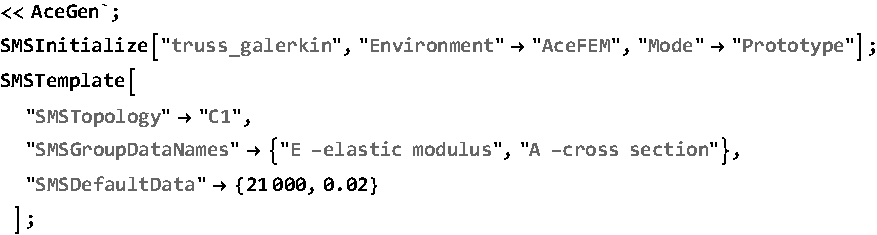
\includegraphics{figures/acegen_input_1}
	\caption{First input}
	\label{fig:first_input}
\end{figure}

Loading the \textit{AceGen} package and initializing constants.


\begin{figure}[htb]
	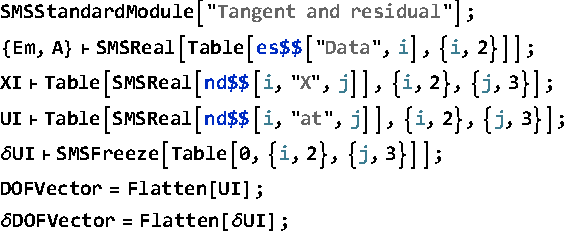
\includegraphics{figures/acegen_input_2}
	\caption{Picking a subroutine and defining variables}
	\label{fig:subroutine}
\end{figure}

\textit{nd\$\$} denotes the nodal data, and \textit{es\$\$} denotes the element structure.
The initialized variational quantities only find use in the standard Galerkin Method.  

\begin{figure}[htb]
	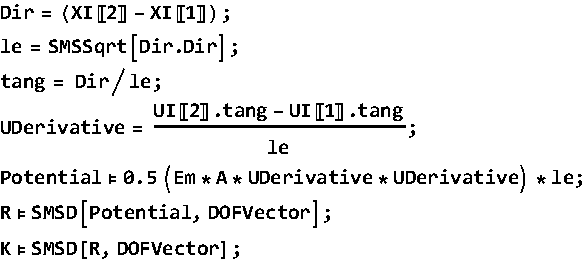
\includegraphics{figures/potentialcode}
	\caption{Main Code for the Potential}
	\label{fig:potential}
\end{figure}
Figure (\ref{fig:potential}) shows the constitutive law, vector \textbf{R}, and matrix \textbf{K}.

\clearpage

\begin{figure}[htb]
	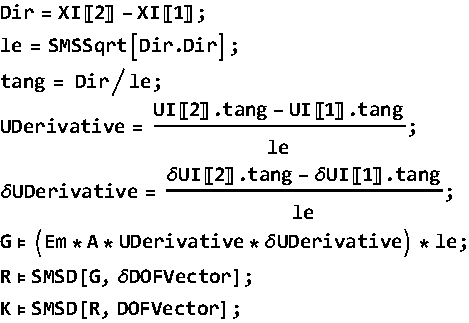
\includegraphics{figures/galerkincode}
	\caption{Main Code for the Standard Galerkin Method}
	\label{fig:galerkin}
\end{figure}

The Standard Galerkin Method uses variational quantities or \textit{trial functions}.

\begin{figure}[htb]
	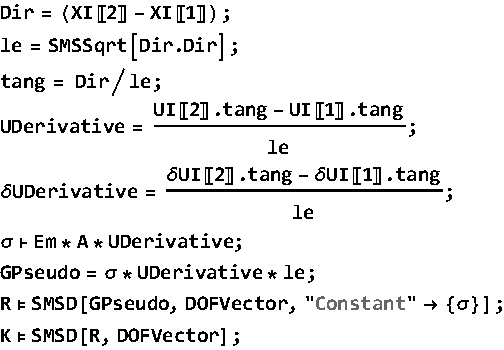
\includegraphics{figures/pseudopotcode}
	\caption{Main Code for the Pseudo Potential}
	\label{fig:pseudo_potential}
\end{figure}

In the Pseudo Potential, a differentiation exception as mentioned in (\ref{eq:pseudoexception}) is used.

\begin{figure}[htb]
	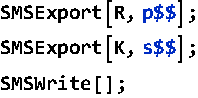
\includegraphics{figures/acegen_input_4}
	\caption{Export}
	\label{fig:Export}
\end{figure}

Lastly, the element is finalized and the element matrices \textbf{R} and \textbf{K} are exported to the fields \textit{p\$\$}, the element load vector, and \textit{s\$\$}, the element stiffness matrix, in \textit{AceFEM}.

\newpage
\section{AceFEM examples}

\begin{figure}[htb]
	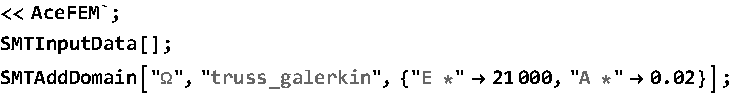
\includegraphics{figures/acefem_input_0}
	\caption{AceFEM system}
	\label{fig:AceFEM First Steps}
\end{figure}

\textit{AceFEM} is initialized and a domain is created. 

\begin{figure}[htb]
	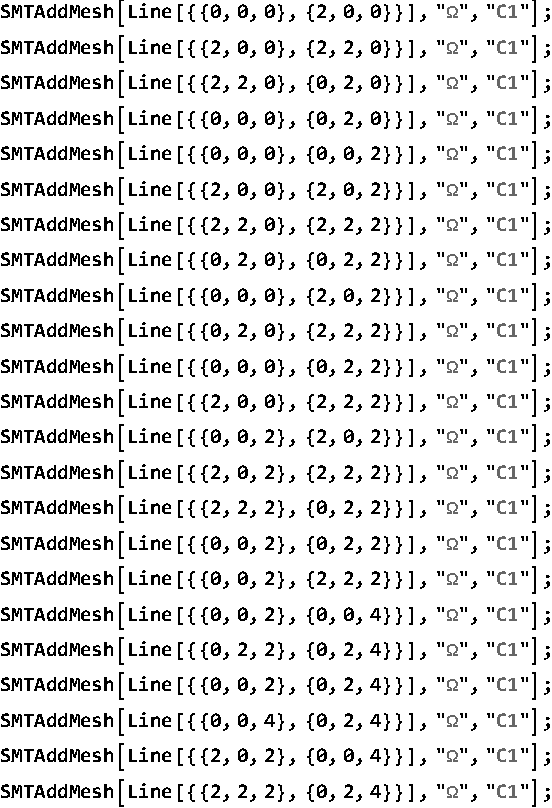
\includegraphics{figures/acefem_input_1}
	\caption{AceFEM system}
	\label{fig:Meshing}
\end{figure}

This mesh is done manually by generating lines with the given element type \textit{C1} on domain \textit{$\Omega$}. A visual example is provided in Figures (\ref{fig:mesh}) and (\ref{fig:def_mesh}).
\clearpage

\begin{figure}[htb]
	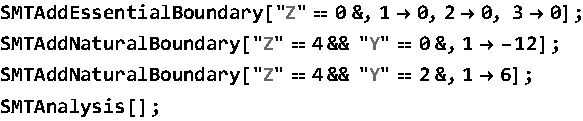
\includegraphics{figures/acefem_input_2}
	\caption{Boundary Conditions And Calculus Phase}
	\label{fig:bound}
\end{figure}

Boundary conditions are applied where necessary, and \textit{AceFEM} is tasked to proceed to calculations.

\begin{figure}[htb]
	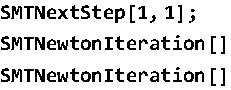
\includegraphics{figures/acefem_input_3}
	\caption{The Last Input: Newton Iterations }
	\label{fig:newton}
\end{figure}

The problem is analyzed by setting the load factor to one, and performing two Newton steps, which is sufficient for a linear problem.

\begin{figure}
	\begin{subfigure}[b]{0.4\textwidth}
		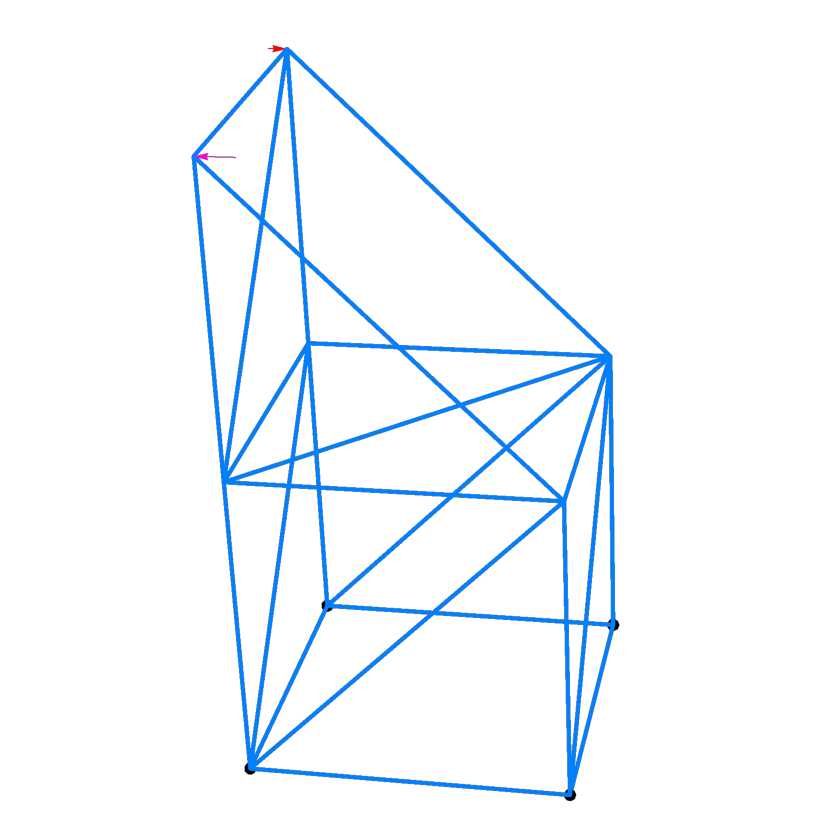
\includegraphics[width=\textwidth]{figures/undeformed}
		\caption{Undeformed mesh}
		\label{fig:mesh}
	\end{subfigure}
	%
	\begin{subfigure}[b]{0.4\textwidth}
		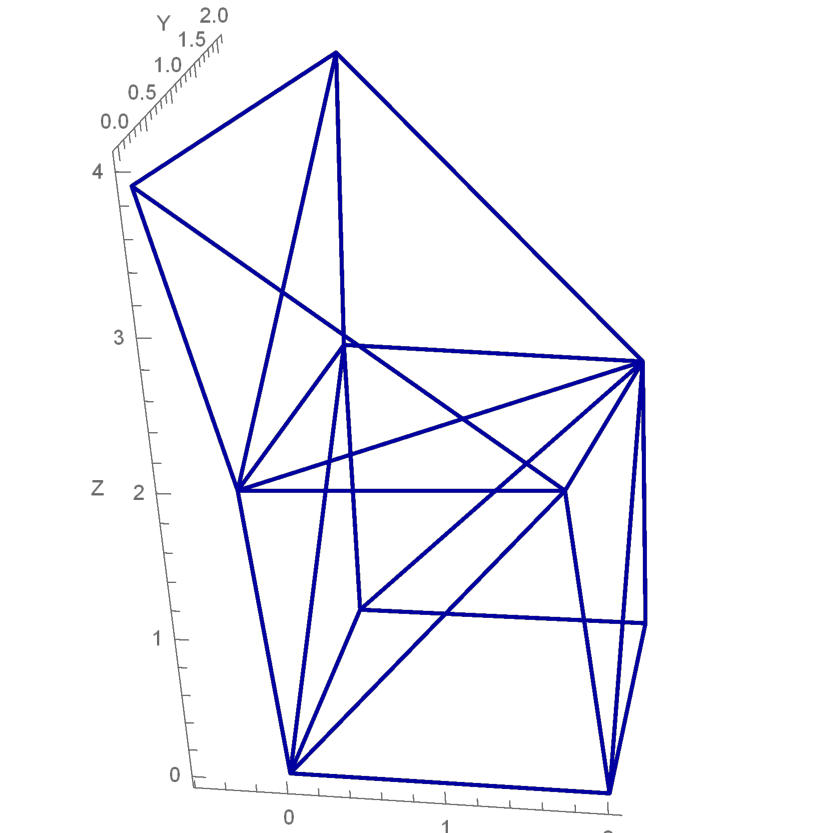
\includegraphics[width=\textwidth]{figures/deformed}
		\caption{Deformed mesh}
		\label{fig:def_mesh}
	\end{subfigure}
	\\ \vspace{5mm}The 2 Figures above show the results of the aforementioned code.
	
\end{figure}



